\section{Algoritmo di Hoshen-Kopelman}
L’algoritmo di Hoshen-Kopelman consente di etichettare in un solo passaggio tutti i cluster connessi presenti in una griglia binaria. Nel mio codice ho diviso il lavoro in due parti principali:
\begin{enumerate}
	\item La funzione \texttt{hk76} attraversa l’intera matrice, attribuendo a ciascun sito occupato un’etichetta.
	\item La funzione \texttt{hkclass} tiene conto del rank di ciasuna label
\end{enumerate} 
In particolare, per ogni sito, la funzione \texttt{hk76} decide l’etichetta da assegnare controllando il vicino sinistro e quello superiore. Data la seguente matrice bidimensionale (15x15)
\begin{figure}[H]
	\centering
     \scriptsize % Riduce la dimensione del testo
	\setlength{\tabcolsep}{5.5pt} % Riduce lo spazio tra le colonne
	\renewcommand{\arraystretch}{1.3} % Riduce lo spazio verticale tra le righe
	\begin{minipage}{0.45\textwidth}
		\centering
		\begin{tabular}{|*{15}{c|}}
			\hline
			0 & 1 & 0 & 0 & 1 & 1 & 0 & 0 & 0 & 1 & 0 & 1 & 0 & 1 & 0 \\
			\hline
			0 & 1 & 1 & 0 & 0 & 0 & 1 & 0 & 0 & 1 & 1 & 1 & 1 & 1 & 1 \\
			\hline
			0 & 1 & 0 & 0 & 0 & 1 & 1 & 1 & 1 & 0 & 0 & 1 & 0 & 0 & 0 \\
			\hline
			1 & 0 & 1 & 0 & 1 & 0 & 1 & 0 & 0 & 0 & 1 & 0 & 0 & 0 & 0 \\
			\hline
			0 & 1 & 0 & 1 & 1 & 0 & 1 & 0 & 0 & 0 & 1 & 0 & 0 & 1 & 0 \\
			\hline
			0 & 0 & 1 & 1 & 1 & 1 & 1 & 0 & 1 & 1 & 1 & 1 & 1 & 0 & 1 \\
			\hline
			0 & 0 & 1 & 1 & 1 & 0 & 0 & 0 & 0 & 1 & 1 & 1 & 1 & 0 & 1 \\
			\hline
			0 & 1 & 0 & 1 & 1 & 1 & 1 & 0 & 1 & 1 & 1 & 1 & 0 & 1 & 0 \\
			\hline
			0 & 1 & 0 & 0 & 1 & 1 & 0 & 0 & 1 & 1 & 1 & 0 & 0 & 0 & 1 \\
			\hline
			1 & 0 & 0 & 0 & 0 & 0 & 0 & 0 & 1 & 0 & 0 & 0 & 0 & 1 & 0 \\
			\hline
			0 & 0 & 0 & 0 & 1 & 0 & 1 & 0 & 1 & 1 & 0 & 1 & 1 & 1 & 1 \\
			\hline
			1 & 1 & 0 & 0 & 0 & 1 & 0 & 1 & 0 & 1 & 1 & 1 & 1 & 1 & 1 \\
			\hline
			1 & 1 & 1 & 0 & 0 & 1 & 1 & 0 & 1 & 0 & 0 & 1 & 0 & 0 & 0 \\
			\hline
			0 & 1 & 0 & 1 & 0 & 1 & 1 & 1 & 0 & 1 & 0 & 0 & 0 & 1 & 1 \\
			\hline
			1 & 1 & 1 & 1 & 0 & 0 & 0 & 1 & 1 & 0 & 0 & 1 & 0 & 1 & 0 \\
			\hline
		\end{tabular}
 	\end{minipage}
	\hfill
	\begin{minipage}{0.5\textwidth}
		\centering
		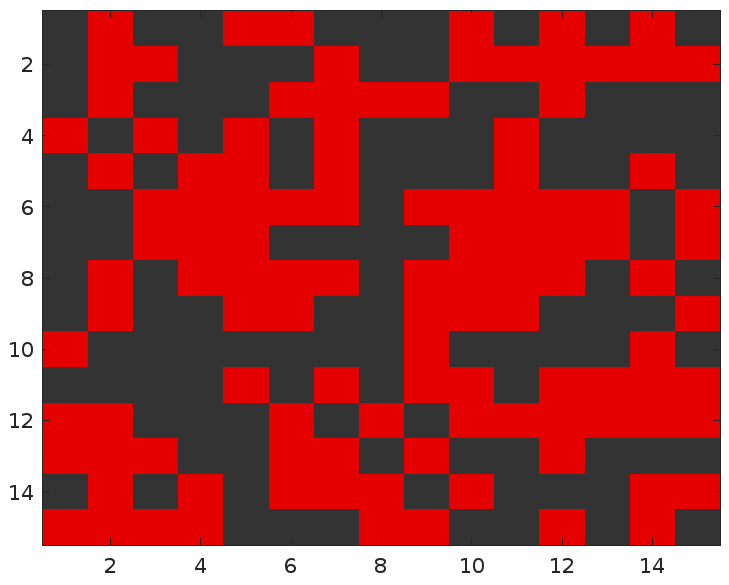
\includegraphics[width=\linewidth]{images/basegrid}
		\label{fig:basegrid}
	\end{minipage}
\end{figure}

L'algoritmo labellerà i siti colorati nel seguente modo
\begin{figure}[H]
	\centering
	\scriptsize % Riduce la dimensione del testo
	\setlength{\tabcolsep}{3.5pt} % Riduce lo spazio tra le colonne
	\renewcommand{\arraystretch}{1.3} % Riduce lo spazio verticale tra le righe
	\begin{minipage}{0.45\textwidth}
		\centering
		\begin{center}
			\begin{tabular}{|*{15}{c|}}
				\hline
				0 & 1 & 0 & 0 & 2 & 2 & 0 & 0 & 0 & 3 & 0 & 4 & 0 & 5 & 0 \\
				\hline
				0 & 1 & 1 & 0 & 0 & 0 & 6 & 0 & 0 & 3 & 3 & 3 & 3 & 3 & 3 \\
				\hline
				0 & 1 & 0 & 0 & 0 & 7 & 6 & 6 & 6 & 0 & 0 & 3 & 0 & 0 & 0 \\
				\hline
				8 & 0 & 9 & 0 & 10 & 0 & 6 & 0 & 0 & 0 & 11 & 0 & 0 & 0 & 0 \\
				\hline
				0 & 12 & 0 & 13 & 10 & 0 & 6 & 0 & 0 & 0 & 11 & 0 & 0 & 14 & 0 \\
				\hline
				0 & 0 & 15 & 13 & 10 & 10 & 6 & 0 & 16 & 16 & 11 & 11 & 11 & 0 & 17 \\
				\hline
				0 & 0 & 15 & 13 & 10 & 0 & 0 & 0 & 0 & 16 & 11 & 11 & 11 & 0 & 17 \\
				\hline
				0 & 18 & 0 & 13 & 10 & 10 & 10 & 0 & 19 & 16 & 11 & 11 & 0 & 20 & 0 \\
				\hline
				0 & 18 & 0 & 0 & 10 & 10 & 0 & 0 & 19 & 16 & 11 & 0 & 0 & 0 & 21 \\
				\hline
				22 & 0 & 0 & 0 & 0 & 0 & 0 & 0 & 19 & 0 & 0 & 0 & 0 & 23 & 0 \\
				\hline
				0 & 0 & 0 & 0 & 24 & 0 & 25 & 0 & 19 & 19 & 0 & 26 & 26 & 23 & 23 \\
				\hline
				27 & 27 & 0 & 0 & 0 & 28 & 0 & 29 & 0 & 19 & 19 & 19 & 19 & 19 & 19 \\
				\hline
				27 & 27 & 27 & 0 & 0 & 28 & 28 & 0 & 30 & 0 & 0 & 19 & 0 & 0 & 0 \\
				\hline
				0 & 27 & 0 & 31 & 0 & 28 & 28 & 28 & 0 & 32 & 0 & 0 & 0 & 33 & 33 \\
				\hline
				34 & 27 & 27 & 27 & 0 & 0 & 0 & 28 & 28 & 0 & 0 & 35 & 0 & 33 & 0 \\
				\hline
			\end{tabular}
		\end{center}
	\end{minipage}
	\hfill
	\begin{minipage}{0.5\textwidth}
		\centering
		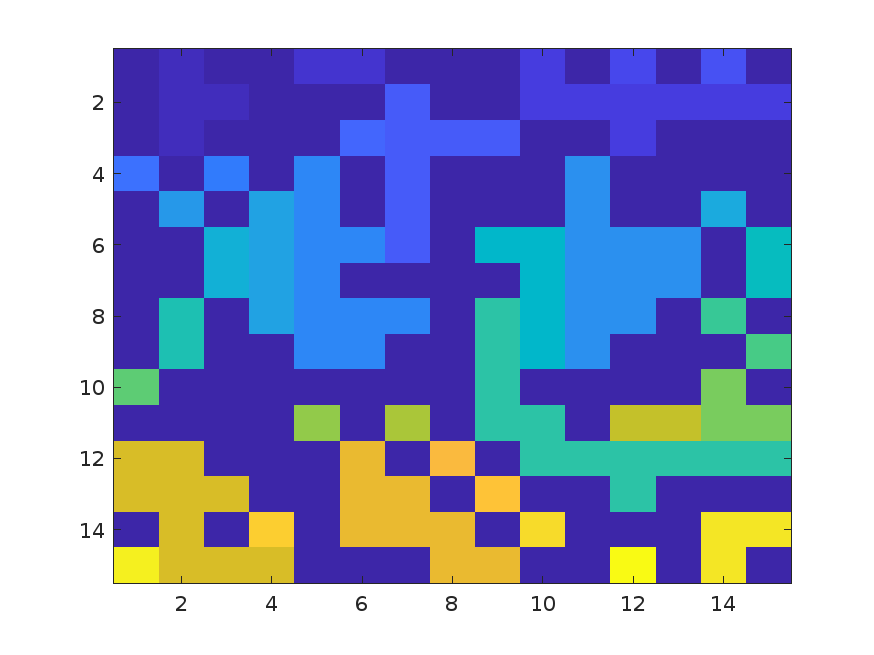
\includegraphics[width=\linewidth]{images/labels}
		\label{fig:basegrid}
	\end{minipage}
\end{figure}
in caso di conflitto tra due etichette differenti, indica a \texttt{hkclass} qual è l’etichetta che dovrà essere "fusa" con quella scelta per il nodo corrente.
Di seguito 

`hkclass` incarna la struttura “union–find” tipica dell’algoritmo: l’array `LofL` contiene, alle posizioni corrispondenti ai root, la dimensione corrente del cluster (valore non negativo); alle posizioni che non sono root è invece memorizzato il puntatore al padre con segno negativo. Quando `badLabel` vale zero la funzione deve soltanto incrementare il contatore del root della componente a cui appartiene `nodeLabel`. Se `nodeLabel` non è un root si risale la catena di puntatori finché non si raggiunge il rappresentante, che è poi il contatore da incrementare.

\begin{tabular}{|c|*{12}{c|}}
	\hline
	\textbf{Label} & 1 & 2 & 3 & 4 & 5 & 6 & 7 & 8 & 9 & 10 & 11 & 12 \\
	\hline
	\textbf{Rank} & 4 & 2 & 10 & -3 & -3 & 24 & -6 & 1 & 1 & -6 & 33 & 1 \\
	\hline
\end{tabular}

\vspace{0.5cm}

% Seconda parte (ID 13–24)
\begin{tabular}{|c|*{12}{c|}}
	\hline
	\textbf{Label} & 13 & 14 & 15 & 16 & 17 & 18 & 19 & 20 & 21 & 22 & 23 & 24 \\
	\hline
	\textbf{Rank} & -10 & 1 & -10 & -11 & 2 & 2 & -11 & 1 & 1 & 1 & -11 & 1 \\
	\hline
\end{tabular}

\vspace{0.5cm}

\begin{tabular}{|c|*{11}{c|}}
	\hline
	\textbf{Label} & 25 & 26 & 27 & 28 & 29 & 30 & 31 & 32 & 33 & 34 & 35 \\
	\hline
	\textbf{Rank} & 1 & -11 & 11 & 8 & 1 & 1 & -27 & 1 & 3 & -27 & 1 \\
	\hline
\end{tabular}



